\section{Visão Geral da Solução}

Usando como base os critérios e características do \textit{design} de linguagens de programação descritos na seção \ref{sec:design_linguagem}, o planejamento da solução foi dado pela definição de alto nível da sintaxe e semântica da linguagem, além da escolha das tecnologias a serem utilizadas na implementação do protótipo.

Já na implementação, o foco foi a construção do interpretador da linguagem proposta no planejamento, iniciando pela criação dos analisadores léxico e sintático, seguidos pela formalização da fase de interpretação. Como base para a implementação, foi principalmente utilizado o livro \textit{Crafting Interpreters} \cite{craftinginterpreters}, além de artigos sobre ECS escritos por Sander Mertens, autor da biblioteca Flecs, e documentação de bibliotecas de ECS, como Flecs \cite{flecs} e Bevy \cite{bevy}.

De modo a permitir uma visão ampla do fluxo de dados do interpretador, desde o código fonte até sua interpretação, a \autoref{fig:diagrama_atividades} apresenta o diagrama de atividades do protótipo proposto pelo trabalho.

\begin{figure}[H]
	\centering
	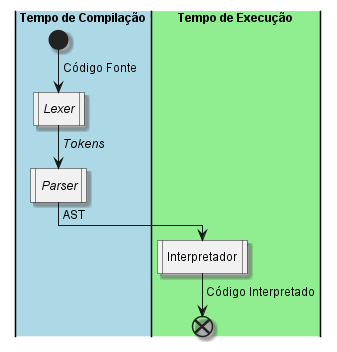
\includegraphics[width=0.25\textheight]{../diagrams/diagrama_atividades.png}
	\caption{Diagrama de atividades efetuadas pelo interpretador.}
	\fonte{Elaboração própria com PlantUML.}
	\label{fig:diagrama_atividades}
\end{figure}

Como ilustrado na \autoref{fig:diagrama_atividades}, nota-se como o fluxo de dados é igual ao de um interpretador tradicional, com apenas as fases de análise léxica, análise sintática e interpretação \cite{craftinginterpreters}. A diferença acontece na implementação por de trás dessas fases, que foram adaptadas para suportar os conceitos de ECS.

Além disso, nota-se como as atividades foram divididas nas faixas de tempo de compilação e tempo de execução. Por mais que tal distinção não terá uso prático no protótipo, ela terá uso para algumas das sugestões de pesquisas futuras, que farão uso das vantagens relacionadas ao tempo de compilação.

Entrando mais a fundo na implementação do interpretador, a \autoref{fig:diagrama_componentes} apresenta o diagrama de componentes do protótipo. Nele, nota-se o agrupamento dos três principais componentes do interpretador\footnote{A relação entre os componentes da implementação e as fases do interpretador é ilustrada na \autoref{tab:terminologia_fases}} — \textit{lexer}, \textit{parser} e interpretador — às suas respectivas fases.

Além disso, nota-se a dependência dos três componentes principais de outros componentes auxiliares, como tanto o \textit{parser} quanto o interpretador dependendo da definição de expressão. A lógica utilizada para agrupar a definição de expressão com o grupo da fase de análise sintática se deve ao fato de que é nela que expressões são criadas, enquanto o interpretador apenas as consome. A mesma lógica se aplica à todos os componentes auxiliares.

\begin{figure}[H]
	\centering
	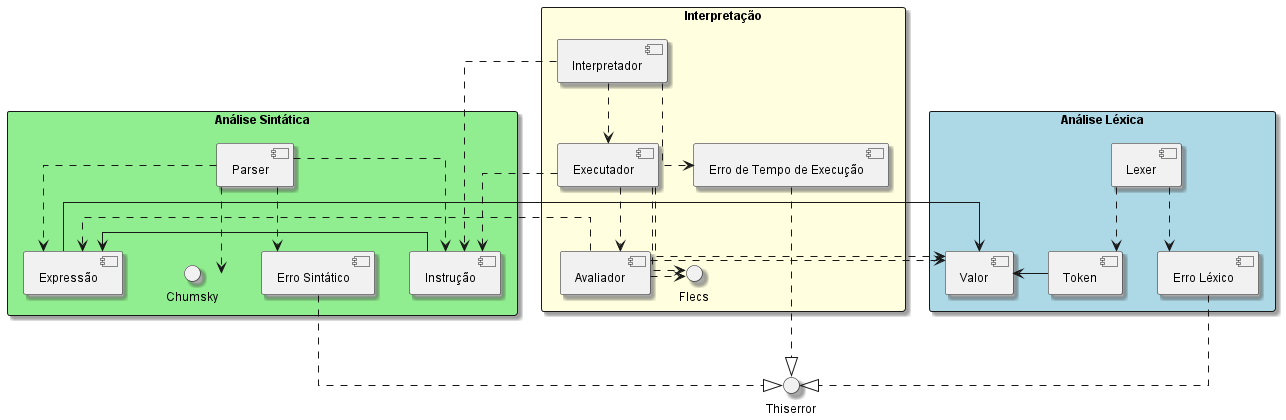
\includegraphics[width=0.65\textheight]{../diagrams/diagrama_componentes.png}
	\caption{Diagrama de componentes do interpretador.}
	\fonte{Elaboração própria com PlantUML.}
	\label{fig:diagrama_componentes}
\end{figure}

Até então, pode-se notar como foram utilizados termos como \textit{lexer} e \textit{parser} ao invés de analisador léxico e analisador sintático, respectivamente. Isso se deve ao fato de que, a partir deste ponto, esses serão os termos utilizados para se referir mais especificamente aos componentes do interpretador, enquanto os termos em português serão utilizados para se referir às fases que caracterizam estes componentes. A \autoref{tab:terminologia_fases} ilustra a diferença de uso entre os termos.

\begin{table}[h]
	\centering
	\caption{Terminologia utilizada para se referir às fases do interpretador e seus componentes.}
	{
		\begin{tabular}{ll}
			\hline
			\textbf{Fase}     & \textbf{Componente}  \\ \hline
			Análise Léxica    & \textit{Lexer}       \\
			Análise Sintática & \textit{Parser}      \\
			Análise Semântica & \textit{Analyzer}    \\
			Interpretação     & \textit{Interpreter} \\ \hline
		\end{tabular}
	}
	\fonte{Elaboração própria com base na terminologia usada em \citeonline{craftinginterpreters}.}
	\label{tab:terminologia_fases}
\end{table}
